\section{Analysis}
In the last section it became evident that the Godot Engine has managed to capture the attention of larger companies, suggesting a degree of relevance in the video game industry.
However, this does not directly address the central question of how relevant the Godot Engine is for indie game developers.
To answer this question effectively, we must first establish a clear definition of what indie game development is.
Just as the definition of a game engine is elusive, so is the definition of indie game development and indie games developed.
The definition used here is from O'Donnell, which states that indie games focus on a few goals and can be developed on a smaller scale in terms of manpower \cite{indie-definition}.
An indie game development team is not financially supported by a larger company.
This is in contrast to AAA titles, which are developed with high budgets and large teams.\\

For this paper, the digital sales platforms Steam and itch.io were selected for investigation.
Firstly, it aligns with a study conducted by Toftedahl and Engström that provides comparative data from 2018 \cite{game-engine-taxonomy}.
Secondly, reference is made to a survey encompassing 2700 video game developers.
Notably, the focus in this paper lies on PC and not on console or mobile games.
This is because the survey ``State of the Game Industry'' from 2022 showed that 65\% are actively developing for PC and 57\% plan to do so in the next project as well \cite{gdc-2023}.
In 2019, a survey involving nearly 4,000 video game developers highlighted that, aside from publisher-owned and individual websites, most games are primarily sold on Steam and itch.io. \cite{gdc-2019}\\

Identifying the game engine used in games available on Steam presents a significant challenge due to a lack of detailed information.
In the paper by Toftedahl and Engström mentioned above, a script was used that matches games with articles on Wikipedia and subsequently assigns game engines.
However, this procedure presents challenges and gaps in the data sets.
This is because not all games possess information about the underlying game engine.
Alternatively, another method involves recognizing the game engines used by analyzing filenames through pattern matching.
The website SteamDB employs this method to deduce the game engines utilized in development \cite{steamdb-tech}.
While this approach provides valuable insights, it is not without its limitations, including the potential for gaps or false positives due to ambiguous filenames.
In this paper, the datasets from SteamDB are used because matching filenames to game engines yield more accurate results than matching the data to Wikipedia articles.
The Godot Engine is not listed in \autoref{table:steam} because the paper providing the comparison data does not list the Godot Engine. \\

\begin{table}[h!]
    \centering
    \begin{tabular}{|c c c c|}
        \hline
        Game Engine & 2018   & 2022    & 2023    \\
        \hline\hline
        Unity       & 25.6\% & 61.22\% & 60.04\% \\
        Unreal      & 13.2\% & 15.91\% & 16.42\% \\
        Source      & 4.0\%  & 0.27\%  & 0.23\%  \\
        CryEngine   & 3.5\%  & 0.23\%  & 0.19\%  \\
        GameBryo    & 3.2\%  & -       & -       \\
        IW          & 2.9\%  & -       & -       \\
        Anvil       & 2.5\%  & 0.05\%  & 0.05\%  \\
        id Tech     & 1.7\%  & 0.18\%  & 0.15\%  \\
        Essence     & 1.1\%  & -       & -       \\
        Clausewitz  & 1.0\%  & 0.03\%  & 0.02\%  \\
        Other       & 48.4\% & 22.17\% & 22.94\% \\
        \hline
    \end{tabular}
    \caption{Percentage of total games identified on Steam (data collected 2022-09-30 and 2023-10-21)}
    \label{table:steam}
\end{table}

\autoref{table:steam} presents the percentages of game engines on Steam for the years 2018, 2022 and 2023.
However, it's important to interpret this comparison cautiously, as two different methods were employed.
The data from 2018 was collected using the Wikipedia method, while the data from 2022 and 2023 was collected using the pattern matching method.
It is also difficult to say whether the newer method can attribute more game engines or simply more games were created using a particular game engine.
To illustrate, consider Unity, which has 35.62\% more share of all identified games from 2018 to 2022.
This could be explained by the pattern matching method capturing more games.
However, it could also be the case that more games in general have been created using the Unity game engine.\\

At the time of the collected data in 2022, 1.15\% of all games created with the Godot Engine were identified.
However, in 2023, this percentage increased to 1.44\%.
Compared to the other game engines on SteamDB, the Godot Engine ranks 6th out of 65 recognized game engines.
This ranking suggests a noteworthy level of relevance in the video game industry for the Godot Engine, given its relatively high position among recognized game engines.
In addition to that it is important to understand that the percentages from \autoref{table:steam} represent lower bounds.
Particularly in the case of the Godot engine, there could be a lot more games.
This is due to the fact that the Godot Engine allows for the export of executables without a recognizable filename signature, making them unidentifiable by the SteamDB algorithm.
Consequently, only a subset of games with specific filename patterns can be matched. \\

\begin{figure}[h!]
    \begin{center}
        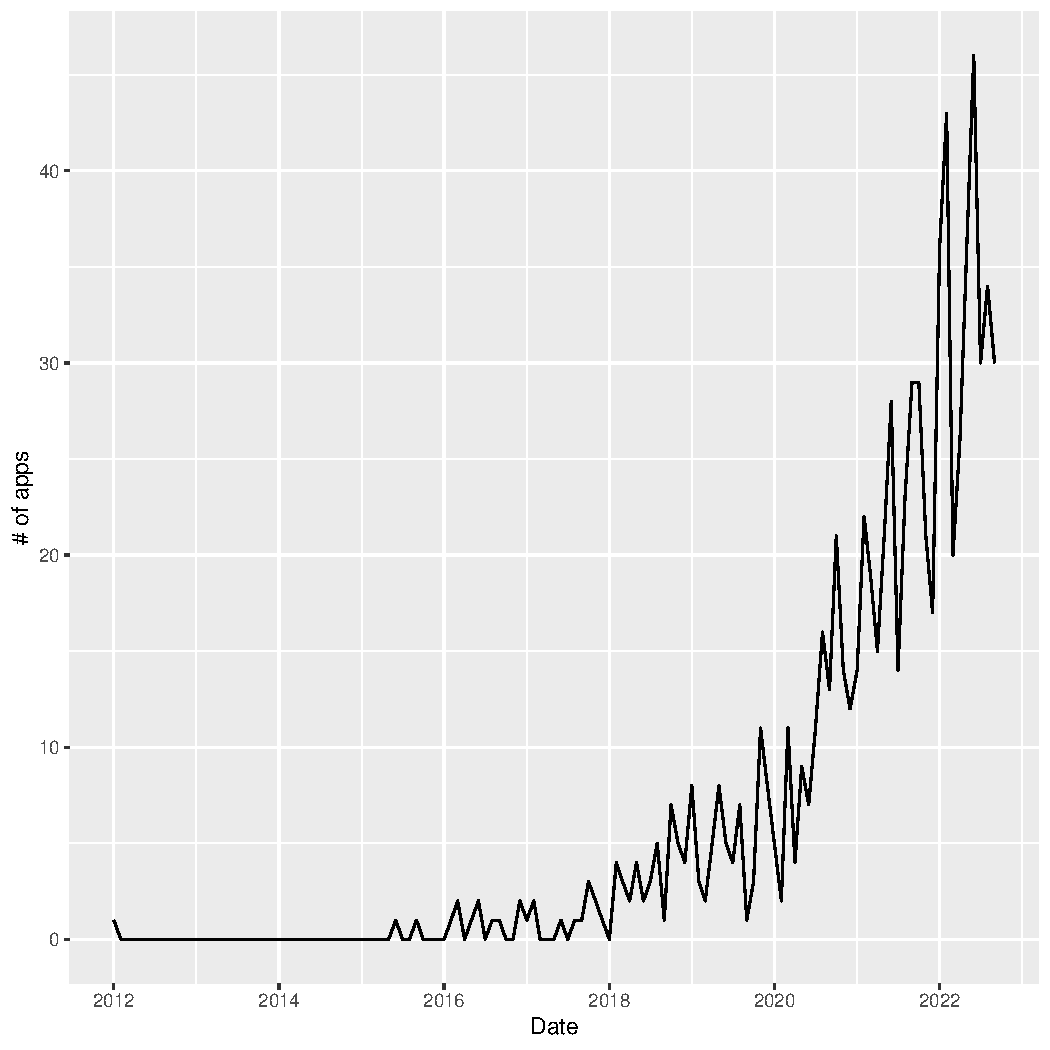
\includegraphics[width=1\columnwidth]{figures/godot-graph.pdf}
        \caption{\label{fig:godot-graph} Number of released Apps on Steam per month}
    \end{center}
\end{figure}

An examination of the monthly app releases depicted in \autoref{fig:godot-graph}, a clear trend emerges: in 2020, there was a significant increase in the number of released games.
This increase in game releases prompts further investigation to understand the underlying reasons.
Prior to conducting a more in-depth analysis of the underlying reasons, we first draw a parallel by comparing the data from itch.io.
In contrast to Steam, the digital sales platform itch.io predominantly showcases indie games, aligning with the specific focus of this paper.
Unlike Steam, itch.io possesses an official statistics website that provides information on game engines \cite{itchio-engines}.
However, it's essential to acknowledge that this data might be incomplete due to its reliance on self-reporting.
Therefore, there may be gaps or inaccuracies in the information, a limitation inherent to self-reported data. \\

\begin{table}[h!]
    \centering
    \begin{tabular}{|c c c c|}
        \hline
        Game Engine & 2018   & 2022                                                & 2023                                                \\
        \hline\hline
        Unity       & 47.3\% & $\textcolor{ForestGreen}{\blacktriangleup 49.75\%}$ & $\textcolor{red}{\blacktriangledown 46.33\%}$       \\
        Construct   & 12.3\% & $\textcolor{ForestGreen}{\blacktriangleup 13.12\%}$ & $\textcolor{ForestGreen}{\blacktriangleup 13.82\%}$ \\
        GameMaker   & 11.0\% & $\textcolor{red}{\blacktriangledown 7.32\%}$        & $\textcolor{red}{\blacktriangledown 6.95\%}$        \\
        Twine       & 6.2\%  & $\textcolor{red}{\blacktriangledown 5.35\%}$        & $\textcolor{ForestGreen}{\blacktriangleup 6.03\%}$  \\
        RPG Maker   & 3.9\%  & $\textcolor{red}{\blacktriangledown 2.74\%}$        & $\textcolor{ForestGreen}{\blacktriangleup 2.76\%}$  \\
        Bitsy       & 3.3\%  & $\textcolor{red}{\blacktriangledown 3.11\%}$        & $\textcolor{ForestGreen}{\blacktriangleup 3.18\%}$  \\
        PICO-8      & 2.9\%  & $\textcolor{red}{\blacktriangledown 2.68\%}$        & $\textcolor{red}{\blacktriangledown 2.60\%}$        \\
        Unreal      & 2.8\%  & $\textcolor{ForestGreen}{\blacktriangleup 2.92\%}$  & $\textcolor{ForestGreen}{\blacktriangleup 3.01\%}$  \\
        Godot       & 2.5\%  & $\textcolor{ForestGreen}{\blacktriangleup 5.55\%}$  & $\textcolor{ForestGreen}{\blacktriangleup 7.51\%}$  \\
        Ren'Py      & 2.0\%  & $\textcolor{red}{\blacktriangledown 1.93\%}$        & $\textcolor{ForestGreen}{\blacktriangleup 2.07\%}$  \\
        Other       & 5.9\%  & $\textcolor{red}{\blacktriangledown 5.55\%}$        & $\textcolor{ForestGreen}{\blacktriangleup 5.75\%}$  \\
        \hline
    \end{tabular}
    \caption{Percentage of total games identified on itch.io (data collected 2022-09-30 and 2023-10-21)}
    \label{table:itch}
\end{table}

Similar to Steam, the data from itch.io can be compared to the 2018 reference paper using the most current data available from 2022 and 2023.
The consistent data collection method allows for direct comparisons, as illustrated in \autoref{table:itch}.
Game engines that have experienced an increase in their percentage of total games developed between 2018 and 2023 are highlighted in green, indicating a positive trend.
Conversely, game engines that have seen a decrease are highlighted in red, suggesting a decline in their usage over the same period.
Upon comparing the data presented in \autoref{table:steam} and \autoref{table:itch}, Unity stands out as a prevalent game engine.
In both 2022 and 2023, Unity consistently constitutes over half of all games on Steam and nearly half on itch.io.
This dominance is particularly striking when considering the second-ranking game engines, which represent approximately 16\% of games on Steam and roughly 14\% on itch.io in 2023.
A similar trend can be observed for 2022. \\

It can also be seen that besides Unity only three other game engines have consistently gained popularity on itch.io.
These three game engines are Construct, Unreal and Godot Engine.
Construct is a game engine primarily aimed at non-programmers.
With the help of visual programming, it is intended to make it easier for novice programmers to get started.
The notable increase in its percentage of games may be attributed to the appeal of game development to a broader audience with limited coding expertise.
However, this is only an assumption that needs to be investigated further. \\

While the Unreal Engine prominently appears as the second most used game engine on Steam, its presence on itch.io has seen only marginal growth over the past four to five years. 
This is particularly interesting as it suggests that the Unreal Engine holds a limited relevance among indie game developers.
The Unreal Engine is often referred to as the game engine for AAA games \cite{unreal-tripple-a-yager, unreal-tripple-a-india}.
This could be one of the reasons why indie game developers have less interest in this game engine. \\

The Godot Engine has gained a lot of popularity in the last four years.
If you look at the underlying data, it becomes clear that the Godot Engine has more than double the percentage share than before.
To be able to analyze the data even further, a separate script was written, which saves the games from itch.io with their release date as a CSV file \cite{github-trend-itch}.
It should be mentioned that not all games could be fetched with this script.
Despite the missing data sets of up to about 10\%, a trend plot for the game engines from \autoref{table:itch} can still be created.

\begin{figure}[h!]
    \begin{center}
        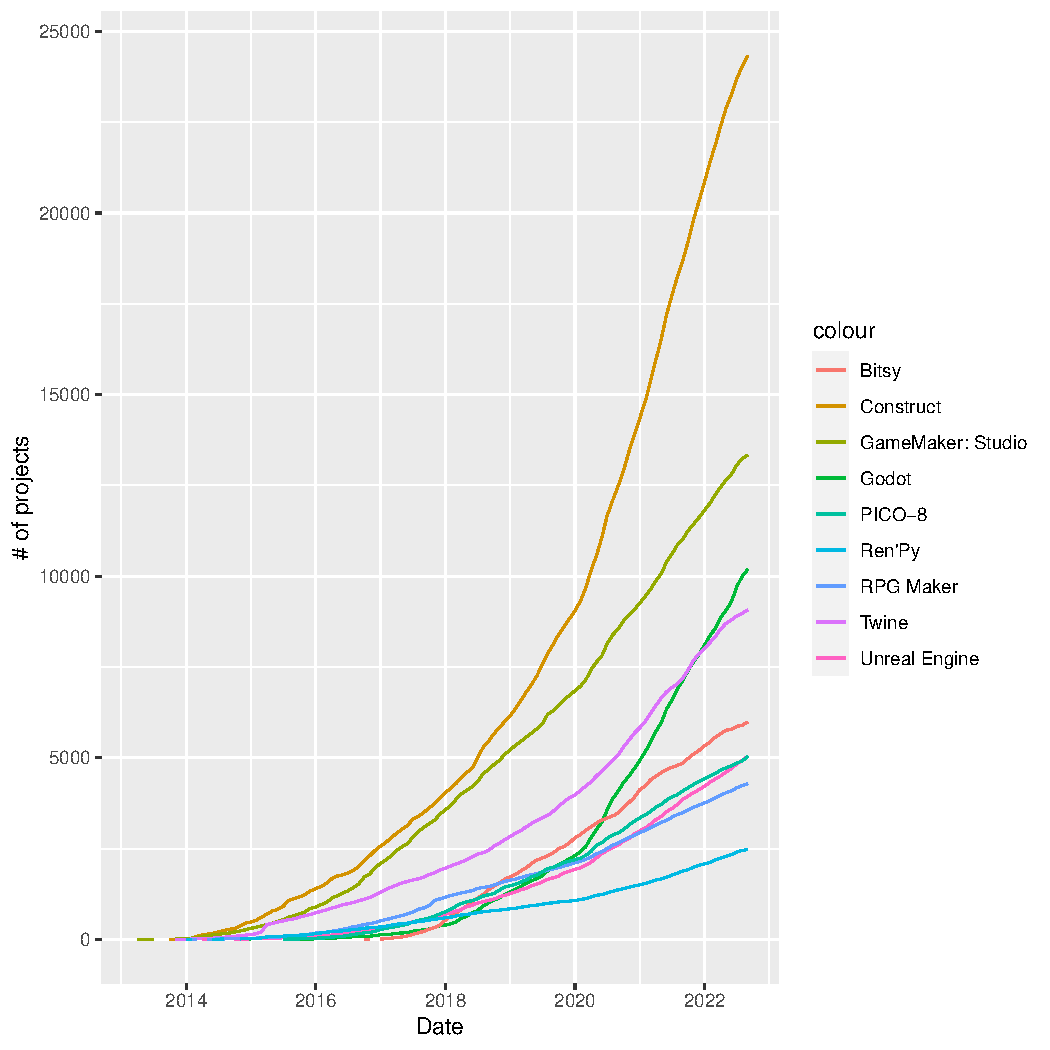
\includegraphics[width=1.1\columnwidth]{figures/trend-graph.pdf}
        \caption{\label{fig:trend-graph} Cumulative sum of the number of projects on itch.io}
    \end{center}
\end{figure}

This graph is shown in \autoref{fig:trend-graph}.
However, Unity has so many projects that the details in the graph would be lost for the other game engines.
For this reason, Unity is not present in the graph.
It is clear to see that the Godot Engine has gained a lot of popularity in 2020, overtaking Bitsy and Twine.
The important observation that emerges here is that both on Steam and on itch.io, more games have been released using the Godot Engine as of 2020.
The reason that more games are released on both platforms may be because developers offer their games for sale on multiple platforms.
Yet, it is quite difficult to determine why exactly the Godot Engine has increased so much in popularity from the beginning of 2020.
This is because there can be numerous factors.
Likewise, important events may have taken place before 2020 that just took longer to make themselves noticeable.
Therefore, only assumptions can be made about the growth in terms of usage on itch.io.
The analysis in this form also reaches its limits, because it is based on the number of games published.
This is because neither the quality nor the number of games published per publisher can be determined.
It is also difficult to say how high the percentage of actual indie game studios is, because not every publisher was analyzed individually.

\begin{table}[h!]
    \centering
    \begin{tabular}{|c c c c c|}
        \hline
        Game Engine & 2020   & 2021                                               & 2022                                               & 2023                                             \\
        \hline\hline
        Unity       & 62.2\% & $\textcolor{red}{\blacktriangledown 61.6\%}$       & $\textcolor{red}{\blacktriangledown 61.1\%}$       & $\textcolor{red}{\blacktriangledown 59\%}$       \\
        Godot       & 12.2\% & $\textcolor{ForestGreen}{\blacktriangleup 13.1\%}$ & $\textcolor{ForestGreen}{\blacktriangleup 15.6\%}$ & $\textcolor{ForestGreen}{\blacktriangleup 19\%}$ \\
        GameMaker   & 10.9\% & $\textcolor{red}{\blacktriangledown 8.9\% }$       & $\textcolor{red}{\blacktriangledown 6.1\%}$        & $\textcolor{red}{\blacktriangledown 5\%}$        \\
        Unreal      & -      & 4.2\%                                              & $\textcolor{ForestGreen}{\blacktriangleup 4.8\%}$  & -                                                \\
        Construct   & 1.7\%  & $\textcolor{ForestGreen}{\blacktriangleup 2.4\%}$  & $\textcolor{red}{\blacktriangledown 1.7\%}$        & -                                                \\
        Stencyl     & 0.1\%  & 0.1\%                                              & -                                                  & -                                                \\
        Other       & 12.9\% & $\textcolor{red}{\blacktriangledown 6.5\%}$        & $\textcolor{ForestGreen}{\blacktriangleup 7.0\%}$  & $\textcolor{ForestGreen}{\blacktriangleup 17\%}$ \\
        No engine   & -      & 3.1\%                                              & $\textcolor{ForestGreen}{\blacktriangleup 3.7\%}$  & -                                                \\
        \hline
    \end{tabular}
    \caption{Used game engines by GMTK Game Jam participants over the years \cite{gmtk-twitter}}
    \label{table:gmtk}
\end{table}

On itch.io there are many games, which were created during a game jam.
Game jams are defined as follows:
\blockquote{A game jam is an accelerated opportunistic game creation event where a game is created in a relatively short timeframe exploring given design constraint(s) and end results are shared publically \cite{game-jam-definition}.}
With around 18,000 - 22,000 participants and around 5,000 - 6,000 submissions, GMTK Game Jam is the largest past game jam event on itch.io \cite{itch-past-jams}.
\autoref{table:gmtk} shows the game engines used by participants in the events from 2020 to 2022.
This table is clearly showing that the Godot Engine is the only game engine from the table to outperform the usage of the previous year two years in a row.
This could be a clue that game jams on itch.io have ensured that the Godot Engine continues to gain relevance.
However, this is also just an assumption.
It is not far-fetched that a general popularity of a game engine also ensures that it is used more often in game jams.\\

To make better assumptions, the Godot Engine can only be compared to other game engines that have gained popularity on itch.io.
The Godot Engine can be classified as a general-purpose game engine, as it covers a wide range of game genres.
According to Toftedahl and Engström, this puts it in the same category as the Unreal Engine and Unity.
Construct, on the other hand, is a special purpose game engine.
In the introduction, it was already explained that game engines should be compared with each other in terms of a specific purpose.
For this reason, Construct should not be included in a comparison.
For such a comparison, a feature matrix, benchmarks or other technical aspects would be interesting.
Unfortunately, this is beyond the scope of this paper and would need to be explored separately.
In this paper, the focus is specifically on the Godot Engine and its importance to the indie game industry.
However, this work can provide the basis for which game engines should be compared with each other with regard to the indie game industry.\\

To explore more about the Godot Engine, the Godot Community Poll from 2022 was examined \cite{godot-poll-results}.
This survey contains 5315 answers with a different set of questions.
When asked about previous experience with other game engines, the top three were Unity (51\%), Other third party engine (30.6\%), and GameMaker (22\%).
With Unity having a strong presence on both Steam and itch.io, it seems natural that developers would have been in contact with the game engine in advance.
It is difficult to make a correct statement about other third party engines, because the game engine would have to be specified for that.
However, a statement, or rather an assumption, can be made about GameMaker.
If you take a closer look at \autoref{table:gmtk}, it becomes clear that GameMaker is the only game engine that has lost an extremely large percentage.
It could therefore be possible that these developers have switched from GameMaker to the Godot Engine.\\

If we look at the data for the usage of the Godot Engine in the poll, we can see that 56.56\% primarily use the Godot Engine for 2D game development.
This is in contrast to the primary usage of 35.22\% in 3D game development.
It can be said that the Godot Engine has the possibility to develop 2D, 3D and especially XR, but it is primarily used for 2D.
This could have several causes.
On one hand, the Godot Engine could provide more functionality for 2D game development than 3D game development.
On the other hand, oftentimes the workload for 3D game development is higher than for 2D game development.
This workload could be a hurdle for indie game developers, which is why they might prefer 2D game development.\\

That the survey is mainly about indie game developers can be seen from the fact that 84\% stated that they use the Godot Engine as a hobby.
9\%, on the other hand, have stated that they work as a full time indie.
If you go by the definition in this paper, hobby developers also belong to indie game developers.
This is because they focus on a few goals, are not financially supported by larger companies and work in small teams.
That this is the case can be seen from the fact that 97.9\% work on their project alone or in a team of up to five people.
Apart from people who do not earn any money with their games (83.7\%), it can also be clearly seen in this survey that the two most represented digital sales platforms are itch.io (7.1\%) and Steam (6\%).
The fact that itch.io performs better than Steam could be another indication that the Godot Engine is more relevant for indie game developers.
However, this is not necessarily the case because there is no other comparative data from other game engines. \\

Regarding the finding that the Godot Engine has increased in relevance in 2020, data can also be found in the survey.
Most people (22.2\%) had already learned about the Godot Engine in 2019.
However, most of them (21.9\%) only started programming with it in the following year 2020.
This confirms the statement that there may have been important events before 2020 that took longer to convince people to develop.
A possible scenario would be an indie game developer who shares his progress on the Godot Engine in individual videos on YouTube.
These videos may have drawn attention to the Godot Engine in 2019.
Since many people were interested in the game engine, the developer may have made the decision to publish a tutorial in 2020, which motivated many people to start developing in the Godot Engine.
Of course, this is only a scenario, and it does not necessarily have to have the direct cause for this occurrence.
This scenario would probably account for only a small percentage.
The other percentages will probably be combined for completely different reasons.
However, it becomes clear to what extent there may be time shifts.
